\documentclass{standalone}

\usepackage{tikz}
\usetikzlibrary{shapes.geometric, arrows}

\tikzstyle{stylein} = [rectangle, rounded corners, minimum width=2cm, minimum height=1cm,text centered, draw=black, fill=red!30]

\tikzstyle{styleout} = [rectangle, rounded corners, minimum width=2cm, minimum height=1cm,text centered, draw=black, fill=blue!30]

\begin{document}
	
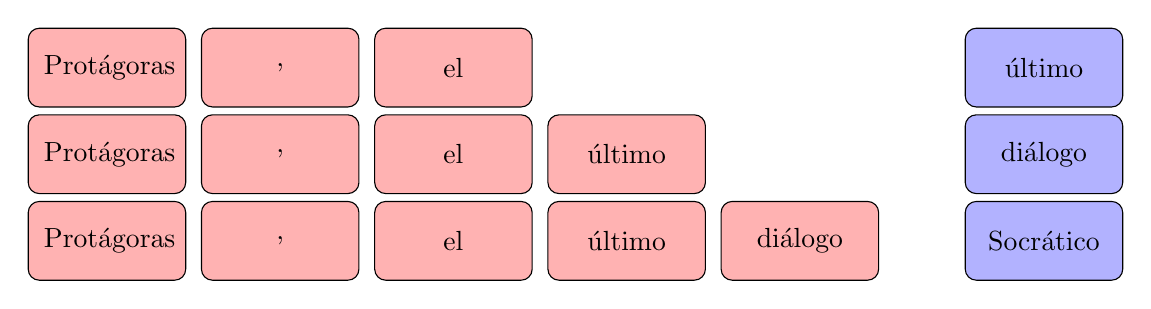
\begin{tikzpicture}[node distance=1.1cm]
%\node (f11) [stylein, text width=1.6cm] {Protágoras};
%\node (f12) [stylein, text width=1.6cm, right of=f11, xshift=1.1cm] {,};
%\node (o1) [styleout, text width=1.6cm, right of=f12, xshift=8.6cm] {el};

\node (f21) [stylein, text width=1.6cm] {Protágoras};
\node (f22) [stylein, text width=1.6cm, right of=f21, xshift=1.1cm] {,};
\node (f23) [stylein, text width=1.6cm, right of=f22, xshift=1.1cm] {el};
\node (o2) [styleout, text width=1.6cm, right of=f23, xshift=6.4cm] {último};

\node (f31) [stylein, text width=1.6cm, below of=f21] {Protágoras};
\node (f32) [stylein, text width=1.6cm, right of=f31, xshift=1.1cm] {,};
\node (f33) [stylein, text width=1.6cm, right of=f32, xshift=1.1cm] {el};
\node (f34) [stylein, text width=1.6cm, right of=f33, xshift=1.1cm] {último};
\node (o3) [styleout, text width=1.6cm, right of=f34, xshift=4.2cm] {diálogo};

\node (f41) [stylein, text width=1.6cm, below of=f31] {Protágoras};
\node (f42) [stylein, text width=1.6cm, right of=f41, xshift=1.1cm] {,};
\node (f43) [stylein, text width=1.6cm, right of=f42, xshift=1.1cm] {el};
\node (f44) [stylein, text width=1.6cm, right of=f43, xshift=1.1cm] {último};
\node (f45) [stylein, text width=1.6cm, right of=f44, xshift=1.1cm] {diálogo};
\node (o3) [styleout, text width=1.6cm, right of=f45, xshift=2cm] {Socrático};

\end{tikzpicture}

\end{document}